\subsection{Data Preprocessing}
Before performing non-negative matrix factorization, the original facial images require preprocessing to reduce the effects of illumination and pixel intensity. This study applied two methods: \textbf{normalization} and \textbf{image size compression}

First, perform pixel value normalization on all images, linearly scaling the grayscale range from [0, 255] to [0, 1]. This ensures images are on the same numerical scale, reducing scale differences between features and thereby stabilizing the algorithm during optimization. It should be noted that this linear scaling does not affect the non-negativity of data; the normalized data still satisfies the non-negativity constraint of NMF.

Second, to reduce computational complexity and unify the input dimensions, images in the ORL dataset were compressed to 30×37 pixels, while those in the YaleB dataset were compressed to 42×48 pixels. The resizing preserved the key facial features while reducing dimensionality, enhancing decomposition efficiency. All images were subsequently flattened into column vectors to form the matrix $V \in \mathbb{R}^{d \times n}$.

According to Gillis (2012), the appropriate preprocessing of the input matrix can improve the posedness of the NMF and lead to more localized and sparser representations\cite{gillis2012sparse}.


\subsection{$L_2$ NMF (Standard NMF)}
$L_2$-NMF is the most common type of Non-negative Matrix Factorization (NMF) and is often called \textbf{Standard NMF}. Given a non-negative data matrix $X \in \mathbb{R}^{m \times n}_{\geq 0},$ for example, consider a data matrix of facial images, where each column represents an image. We want to decompose it into two smaller non-negative matrices:
\begin{align}
    X \approx WH
\end{align}
where \(W \in \mathbb{R}^{m \times k}_{\geq 0}\) is the \textit{basis matrix}, and \(H \in \mathbb{R}^{k \times n}_{\geq 0}\) is the \textit{coefficient matrix}. Intuitively, the basis matrix $W$ contains a set of building blocks, while the coefficient matrix $H$ indicates how these blocks are combined to reconstruct the original data. Due to the non-negativity constraint, “negative bricks” cannot offset other components, making the results more intuitive and easier to interpret \cite{lee1999learning}.  

\subsubsection{Objective function}
To make sure that the reconstructed matrix \(WH\) is close to the original data \(X\), $L_2$-NMF minimizes the Frobenius norm of their difference:
\begin{align}
    \min_{W,H \geq 0} \; \|X - WH\|_F^2
\end{align}
This \textbf{loss function} measures the squared error between the original matrix and the reconstructed one. It's like comparing the pixel differences between two images—the smaller the difference, the better the decomposition effect\cite{lee2001algorithms}.

\subsubsection{Optimization}
Directly solving this problem is difficult, so Lee and Seung \cite{lee2001algorithms} proposed the \textit{Multiplicative Update Rules (MUR)}. These rules update \(W\) and \(H\) iteratively as follows:
\begin{align}
    W_{ij} \leftarrow W_{ij} \frac{(X H^T)_{ij}}{(W H H^T)_{ij}}, \\
    H_{ij} \leftarrow H_{ij} \frac{(W^T X)_{ij}}{(W^T W H)_{ij}}
\end{align}

The update process first calculates the error based on the current decomposition results, then adjusts the values of $W$ and $H$. Since both the numerator and denominator are greater than zero, this update method naturally keep the non-negativity of the matrices. Additionally, Lee \& Seung\cite{lee2001algorithms} proved that this update scheme ensures the error function decreases monotonically until converging to a local optimum.

In the implementation, the maximum number of iterations was set to 5000. The algorithm stops when the sum of parameter updates in $W$ and $H$ becomes smaller than $10^{-10}$ between two consecutive iterations. This setting ensures that the optimization reaches a stable point while avoiding unnecessary computation.


\subsubsection{Advantages and Disadvantages}
$L_2$-NMF, also known as Standard NMF, has both strengths and weaknesses. Since the factorization process is subject to non-negative constraints, the resulting decompositions can be interpreted as additive combinations of the original data. This property ensures that the decomposed results possess excellent interpretability. For instance, in facial image analysis, the basis matrix often represents component-based features such as eyes and noses,  giving an intuitive explanation of how the data is structured \cite{lee1999learning}. Another benefit is that $L_2$-NMF performs well in the areas of dimensionality reduction and feature extraction. It effectively compresses high-dimensional data into a low-dimensional space, thereby reducing computational and storage overhead while preserving the most important patterns within the data \cite{buciu2008nmf}.

On the other hand, $L_2$-NMF also has some limitations. Since the optimization problem is non-convex, the results are sensitive to initialization,the iterative process can only guarantee convergence to a local optimum, different initialization methods may lead to significant variations in results. Secondly, $L_2$-NMF employs the squared error as its loss function, which makes it less robust when handling data with noise or outliers. Even a small number of anomalous samples can significantly impact the factorization results. For this reason, researchers have proposed more robust variants to improve its performance in real-world settings \cite{guan2012online}.


\subsection{$L_{2,1}$-Norm Based NMF}

\subsubsection{Objective Function}

The Objective Function of standard NMF is given by Eq.\eqref{eq.standred NMF}. The normalized NMF method assumes that the noise follows a Gaussian distribution. In the $L_{2,1}$ NMF method, we assume that the noise follows a Laplacian distribution\cite{kong2011robust}.

The main disadvantage of the standard NMF method is that it is greatly affected by outliers, that is, it has poor robustness. Consider the expansion of the objective function of standardized NMF is:

\begin{align}
    ||X-WH||_F^2 = \sum_{i=1}^n||x_i-Wh_i||^2
\end{align}

Any possible outliers will become larger due to the square effect $||x_i-Wh_i||^2$, thus having a greater impact on the final result. Considering that $W$ and $H$ are unknown, the impact of outliers may exceed that of a simple convex optimization problem\cite{kong2011robust}. Therefore, we need to propose stable NMF methods and discuss their stability.

The error equation for method $L_{2,1}$-Norm Based NMF is:

\begin{align}
    ||X-WH||_{2,1} = \sum_{i=1}^n\sqrt{\sum_{j=1}^p(X-WH)_{ji}^2} = \sum_{i=1}^n||x_i-Wh_i||
\end{align}

\subsubsection{Theoretical Robustness View}

The square form of the original error equation is converted into a linear form $||x_i-Wh_i||$ in this method. Therefore, in theory, such a method is less affected by outliers than the standardized NMF method. We propose robust $L_{2,1}$ NMF formulated as:

\begin{align}
    \min_{W,H}||X-WH||_{2,1} \, s.t. W\geq 0, H\geq 0 \label{eq:L21 goal}
\end{align}

$L_{2,1}$ norm is first proposed in article\cite{ding2006r}. It is defined as:

\begin{align*}
    ||A||_{2,1}= \sum_{i=1}^n \sqrt{\sum_{j=1}^p A_{ji}^2} = \sum_{i=1}^n ||a_i||
\end{align*}

where $a_i$ is the $i$-th column of $A$. $a_i$ contribute in the form of vector Euclidean norm. $||\cdot||_{2,1}$ is a vaild norm as it satisfies 3 conditions:

\begin{itemize}
    \item Positive scalability: $||\alpha A||_{2,1} = |\alpha|||A||_{2,1}$
    \item Triangle inequality: $||A+B||_{2,1}\leq ||A||_{2,1} + ||B||_{2,1}$
    \item Existence of a zero vector: if $||A||_{2,1} = 0$, then $A=0$.
\end{itemize}

From a statistical point of view, the method $L_{2,1}$ NMF assumes that the noise follows the Laplace distribution. This distribution is more suitable for scenarios with sparse and large noise. The process of deriving the $L_{2,1}$ objective function from the Laplace noise distribution can be found in the literature\cite{kong2011robust}.

\subsubsection{Optimization Steps}

The main goal of the iterative process of this method is to minimize the equation Eq.\eqref{eq:L21 goal}. Our iterative function is shown as:

\begin{align}
    W_{jk}\;\leftarrow\; W_{jk} \frac{(XDH^T)_{jk}}{(WHDH^T)_{jk}}\\
    H_{ki}\;\leftarrow\; H_{ki} \frac{(W^TXD)_{ki}}{(W^TWHD)_{ki}}
\end{align}

where $D$ is a diagonal matrix with the diagonal elements given by:

\begin{align}
    D_{ii} = 1/\sqrt{\sum_{i=1}^p(X-WH)_{ji}^2} = 1/||x_i-Wh_i||
\end{align}

Here, we introduce a $D$ matrix to adjust the weight of each sample. Samples with larger errors have their weights reduced accordingly. The update steps in this method are very similar to those in standard NMF. Therefore, the cost of this method is also similar to that of standard NMF. The introduction of the $D$ matrix can effectively enhance robustness.

The objective function is monotonically decreasing at each iteration. It also satisfies the KKT condition\cite{kong2011robust}.

For the L$_{2,1}$-NMF algorithm, the maximum iteration number was also set to 5000. The optimization procedure was terminated when the relative change of the objective function between two successive iterations was smaller than $10^{-7}$. This convergence criterion achieves a good balance between numerical stability and computational efficiency.


\subsection{Salt and pepper noise}
Salt and pepper noise is a common type of impulse noise in image processing. Its characteristic is the random appearance of small black (0) and white (255) pixels within the image. This noise is typically caused by sensor defects, data transmission errors, or other hardware issues, and can significantly reduce the clarity of an image by distorting local details. Previous studies have shown that, in face images, the presence of salt and pepper noise can make tasks like reconstruction and feature extraction much more difficult\cite{zhang2015inpainting,alazzeh2018salt}.

In this study, we introduced salt-and-pepper noise into face image datasets to test the robustness of two NMF algorithms under noisy conditions. We set two parameters to control the level and type of noise: $p$ represents the overall percentage of pixels to be altered, $r$ represents the proportion of white (salt) among the replaced pixels, with the remainder being black (pepper). By varying these parameters, we were able to simulate different noise levels and visual patterns.

\begin{figure}[h]
  \centering
  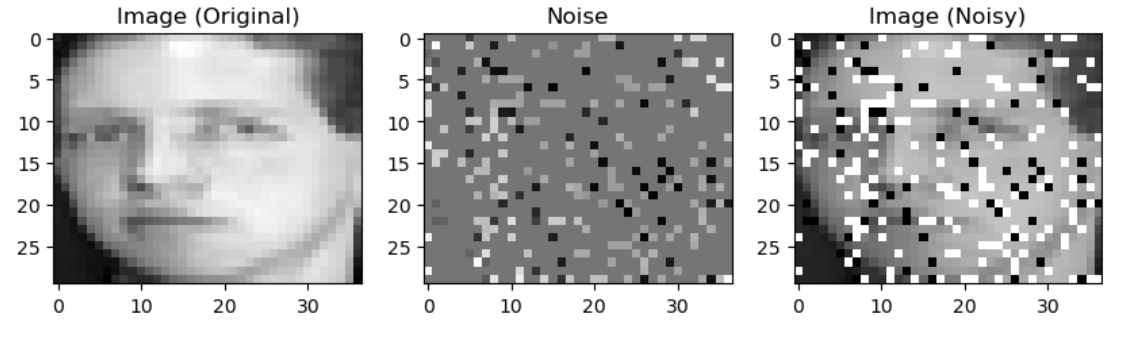
\includegraphics[width=0.85\textwidth]{figure/ORLnoise.png}
  \caption{Example of salt-and-pepper noise applied to an ORL face image.}
  \label{fig:ORLnoise}
\end{figure}
Figure~\ref{fig:ORLnoise} shows an example from the ORL dataset. The left image shows the original image, the middle image displays the added noise layer, and the right image presents the result after noise is added. It can be seen that black and white pixels are randomly distributed across the entire image, causing significant interference to the facial structure.
\begin{figure}[h]
  \centering
  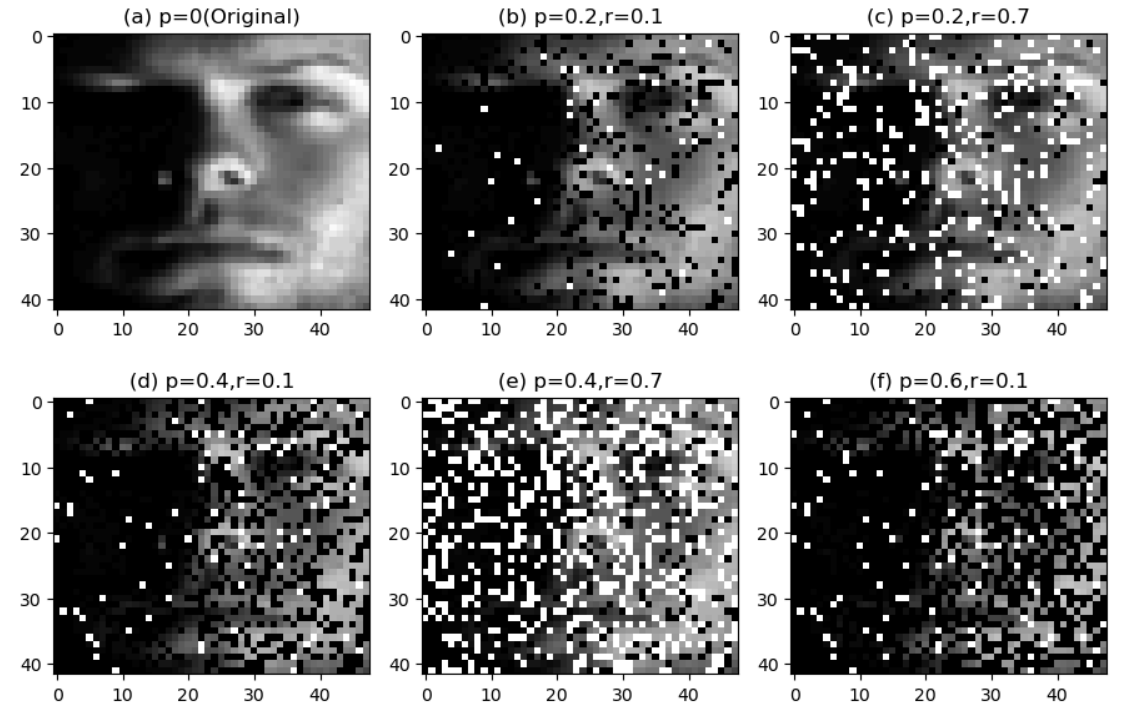
\includegraphics[width=0.9\textwidth]{figure/Yalebnoise.png}
  \caption{Examples of salt-and-pepper noise applied to the YaleB dataset under different parameter settings of $p$ and $r$.}
  \label{fig:Yalebnoise}
\end{figure}

Figure~\ref{fig:Yalebnoise} presents samples from the YaleB dataset under different noise settings. As the value of $p$ increases, the noise becomes denser and more destructive.  Adjusting the value of $r$ alters the ratio of black and white pixels, thereby changing the brightness distribution of the noise. These examples illustrate how salt and pepper noise impacts image appearance under various conditions, providing a basis for evaluating the robustness of the models we applied.